\subsection{Spektrograph}
Der verwendete Spektrograph ist der \textsc{DADOS}--Spektrograph (\ref{fig:dados}).
\begin{figure}[t]
  \centering
  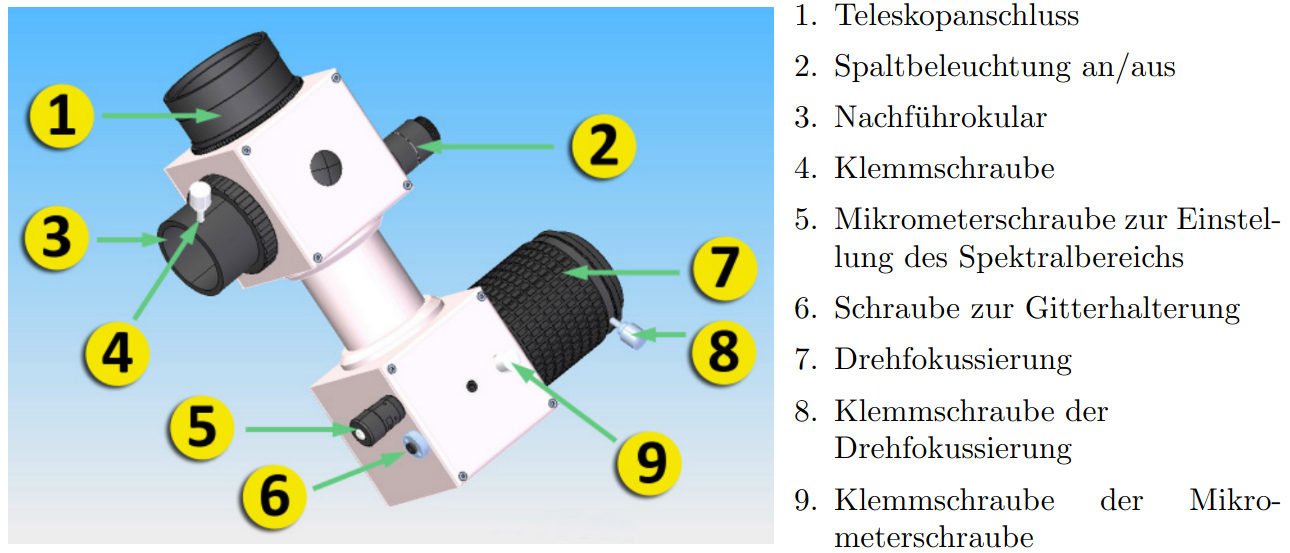
\includegraphics[width=.5\textwidth]{464_dados_spektrograph.png}
  \caption{Der verwendete DADOS--Spektrograph mit Legende.\cite{anleitung464}} \label{fig:dados}
\end{figure}
\begin{figure}[t]
  \centering
  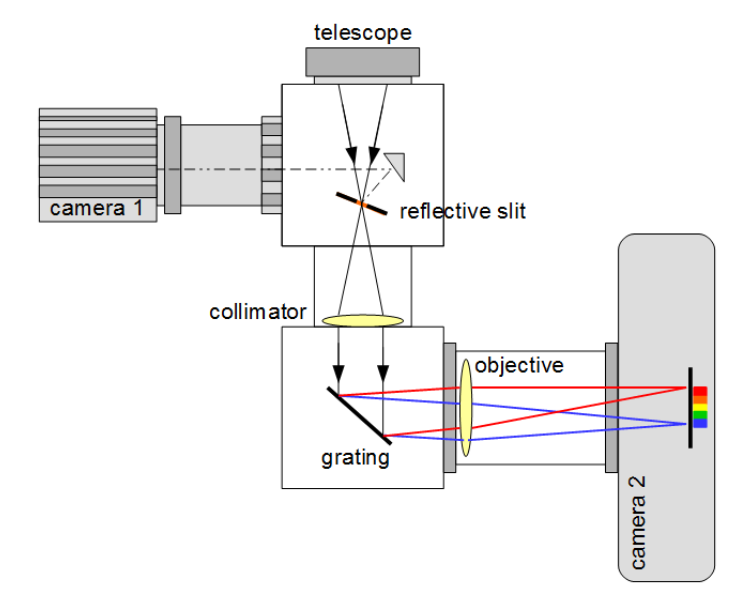
\includegraphics[width=.5\textwidth]{464_dados_schema.png}
  \caption{Schematische Zeichnung des DADOS--Spektrographen.\cite{anleitung464}} \label{fig:dados_schema}
\end{figure}
Eine schematische Zeichnung ist in Abb.\ (\ref{fig:dados_schema}) zu sehen.
Das eingehende Licht vom Teleskop trifft auf einen halbdurchlässigen Spalt, mit dem es sowohl in ein Okular als auch in einen Kollimator geleitet wird.
Hinter dem Kollimator trifft das Licht auf ein Reflexionsgitter, bei dem es in seine Wellenlängen aufgespalten wird.
Mit Hilfe einer CCD kann dieses Licht eingefangen werden und als Absorptionsspektrum ausgelesen werden.
